\chapter{A Car Navigation System Example}\label{app:navigation}

This section presents the requirements for a in-car radio navigation system which supports the Traffic Message Channel (TMC). It forms a running example that serves to illustrate the process described earlier and to introduce elements of the VDM++ modelling language with the Real-time extension VICE. Although the modelling process is described here as though it were a single-pass activity, a real development would usually be iterative. 

%%\section{An informal description}

%%Chapter~\ref{cha:toolbox} provides an interactive and hands-on tour of
%%the tools available for supporting the development of the model.

%%The system is composed of three main clusters of functionality; 
%%\begin{itemize}
%%\item The man-machine interface (MMI) takes care of user interaction such as handling key press input and graphical display output. 
%%\item The navigation is responsible for destination entry, route planning and turn-by-turn guidance. 
%%\item The radio is responsible for basic tuner and volume control as well as handling traffic information from the TMC.
%%\end{itemize}

%%The system must be able to support the following three use cases:

%%\begin{description}
%%\item[Change Volume:] The user turns the rotary button and expects near instant audible feedback form the system. Furthermore, the visual feedback
%%(the volume setting on the screen) should be timely and synchronized with the
%%audible feedback.
%%\item[Address Look-up:] Destination entry is supported by a smart �typewriter� style interface. By turning a knob the user can move from letter to letter; by pressing it the user will select the currently highlighted letter. The map database is searched for each letter that is selected and only those letters in the on-screen alphabet are enabled that are potential next letters in the list.
%%\item[TMC Message Handling:] Digital traffic information is important for in-car radio navigation systems. It enables features such as automatic re-planning of the planned route in case a traffic jam occurs ahead. It is also increasingly important to enhance road safety by warning the driver, for example when a ghost driver is spotted just ahead on the planned route. TMC is such a digital traffic information service.
%%\end{description}

\section{System Overview of the Car Navigation example}

%In Figure~\ref{fig:navigationoverview} an overview of the in-car
%navigation system is shown. Similarily 
Figure~\ref{fig:worldenv}
provides an overview of the \texttt{World} class and the environment
classes. 

%% \begin{figure}[!htb]
%% \begin{center}
%%   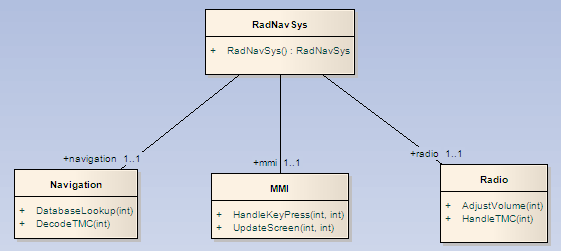
\includegraphics[width=5in]{figures/carnavsys}
%%   \caption[labelInTOC]{Car Navigation System Overview}
%%   \label{fig:navigationoverviewapp}
%% \end{center}
%% \end{figure}

\begin{figure}[!htb]
\begin{center}
  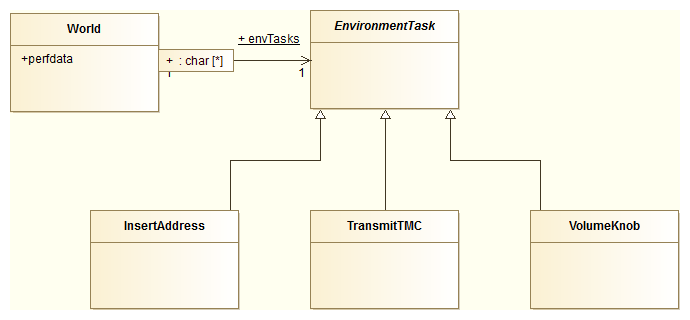
\includegraphics[width=5in]{figures/worldenv}
  \caption[labelInTOC]{Overview of the World and Environment Classes}
  \label{fig:worldenv}
\end{center}
\end{figure}

\section{The Radio Navigation System Class}

The \texttt{RadNavSys} class is the system class that all VDMRT models must include. 

\begin{lstlisting}
system RadNavSys

instance variables
  -- create an MMI class instance
  static public mmi : MMI := new MMI();
  -- define the first CPU with fixed priority 
  -- scheduling and 22E6 MIPS
  CPU1 : CPU := new CPU (<FP>, 22E6);

  -- create an Radio class instance
  static public radio : Radio := new Radio();
  -- define the second CPU with fixed priority 
  -- scheduling and 11E6 MIPS
  CPU2 : CPU := new CPU (<FP>, 11E6);

  -- create an Navigation class instance
  static public navigation : Navigation := new Navigation();
  -- define the third CPU with fixed priority 
  -- scheduling and 113 MIPS
  CPU3 : CPU := new CPU (<FP>, 113E6); 

  -- create a communication bus that links the three 
  -- CPU's together
  BUS1 : BUS := new BUS (<CSMACD>, 72E3, {CPU1, CPU2, CPU3})
\end{lstlisting}

\begin{lstlisting}
operations
  public RadNavSys: () ==> RadNavSys
  RadNavSys () ==
    ( -- deploy mmi on CPU1
      CPU1.deploy(mmi,"MMIT");
      CPU1.setPriority(MMI`HandleKeyPress,100);
      CPU1.setPriority(MMI`UpdateScreen,90);
      -- deploy radio on CPU2
      CPU2.deploy(radio,"RadioT");
      CPU2.setPriority(Radio`AdjustVolume,100);
      CPU2.setPriority(Radio`DecodeTMC,90);
      -- deploy navigation on CPU3
      CPU3.deploy(navigation,"NavT");
      CPU3.setPriority(Navigation`DatabaseLookup, 100);
      CPU3.setPriority(Navigation`DecodeTMC, 90)
      -- starting the CPUs and BUS is implicit
    );
end RadNavSys
\end{lstlisting}

\section{The MMI Class}

\begin{lstlisting}
class MMI

operations
  async 
  public HandleKeyPress: nat * nat ==> ()
  HandleKeyPress (pn, pno) ==
    ( cycles (1E5) skip;
      cases (pn):
        1 -> RadNavSys`radio.AdjustVolume(pno),
        2 -> RadNavSys`navigation.DatabaseLookup(pno)
      end );

  async 
  public UpdateScreen: nat * nat ==> ()
  UpdateScreen (pn, pno) ==
    ( cycles (5E5) skip;
      cases (pn):
        1 -> World`envTasks("VolumeKnob").HandleEvent(pno),
        2 -> World`envTasks("InsertAddress").HandleEvent(pno),
        3 -> World`envTasks("TransmitTMC").HandleEvent(pno)
      end )

end MMI
\end{lstlisting}

\section{The Radio Class}

\begin{lstlisting}
class Radio

operations
  async 
  public AdjustVolume: nat ==> ()
  AdjustVolume (pno) ==
    ( cycles (1E5) skip;
      RadNavSys`mmi.UpdateScreen(1, pno) );

  async 
  public HandleTMC: nat ==> ()
  HandleTMC (pno) ==
    ( cycles (1E6) skip;
      RadNavSys`navigation.DecodeTMC(pno) )

end Radio
\end{lstlisting}

\section{The Navigation Class}

\begin{lstlisting}
class Navigation

operations
  async 
  public DatabaseLookup: nat ==> ()
  DatabaseLookup (pno) ==
    ( cycles (5E6) skip;
      RadNavSys`mmi.UpdateScreen(2, pno) );

  async 
  public DecodeTMC: nat ==> ()
  DecodeTMC (pno) ==
    ( cycles (5E5) skip;
      RadNavSys`mmi.UpdateScreen(3, pno) )

end Navigation
\end{lstlisting}

\section{The Environment Task Class}

\begin{lstlisting}
class EnvironmentTask 

instance variables
  -- use a unique identifier for each generated event
  private num : nat := 0;

  -- we limit the number of inserted stimuli
  protected max_stimuli : nat := 0;

  -- administration for the event traces
  -- e2s is used for all out-going stimuli 
  -- (environment to system)
  -- s2e is used for all received responses 
  -- (system to environment)
  protected e2s : map nat to nat := {|->};
  protected s2e : map nat to nat := {|->}

functions
  -- checkResponseTimes verifies for each received response 
  -- whether or not the elapse time did (not) exceed the 
  -- user-defined limit
  public checkResponseTimes: map nat to nat * 
                             map nat to nat * nat -> bool
  checkResponseTimes (pe2s, ps2e, plim) ==
    forall idx in set dom ps2e &
      ps2e(idx) - pe2s(idx) <= plim
  -- the responses received should also be sent
  pre dom ps2e inter dom pe2s = dom ps2e
  
operations
  public EnvironmentTask: nat ==> EnvironmentTask
  EnvironmentTask (pno) == max_stimuli := pno;

  public getNum: () ==> nat
  getNum () ==
  ( dcl res : nat := num; 
    num := num + 1; 
    return res );

  -- Run shall be overloaded to implement the event generation 
  -- loop towards the system. typically, it starts a periodic 
  -- thread
  public Run: () ==> ()
  Run () == is subclass responsibility;

  public HandleEvent: nat ==> ()
  HandleEvent (pev) == is subclass responsibility;
 
  -- logEnvToSys is used to register when an event was inserted 
  -- into the system. Note that the 'time' keyword refers to 
  -- the internal simulation wall clock of Overture
  public logEnvToSys: nat ==> ()
  logEnvToSys (pev) == e2s := e2s munion {pev |-> time};

  -- logSysToEnv is used to register when an event was received 
  -- from the system. Note that the 'time' keyword refers to the 
  -- internal simulation wall clock of Overture
  public logSysToEnv: nat ==> ()
  logSysToEnv (pev) == s2e := s2e munion {pev |-> time};

  -- getMinMaxAverage calculates the minimum, maximum and 
  -- average response times that were observed during execution 
  -- of the model note that getMinMaxAverage is blocked until 
  -- the number of system responses is equal to the number of 
  -- sent stimuli termination is ensured because only a maximum 
  -- number of stimuli is allowed to be inserted in the system, 
  -- so eventually all stimuli can be processed by the system. 
  -- This method only works when each stimulus leads to exactly 
  -- one response, which is the case in this instance.
  public getMinMaxAverage: () ==> nat * nat * real
  getMinMaxAverage () ==
    ( dcl min : [nat] := nil, 
          max : [nat] := nil, 
          diff : nat := 0;
      for all cnt in set dom s2e do
        let dt = s2e(cnt) - e2s(cnt) in
          ( if min = nil then min := dt
            else (if min > dt then min := dt);
            if max = nil then max := dt
            else (if max < dt then max := dt);
            diff := diff + dt );
      return mk_(min, max, diff / card dom s2e) )

public static IsFinished: () ==> ()
IsFinished() == skip;

sync
  -- getNum is mutually exclusive to ensure unique values
  mutex (getNum);
  -- getMinMaxAverage is blocked until all responses have 
  -- been received
  per getMinMaxAverage => card dom s2e >= max_stimuli;

  per IsFinished => #fin(logSysToEnv) > 0;

end EnvironmentTask
\end{lstlisting}

\section{The Insert Address Class}

\begin{lstlisting}
class InsertAddress
  is subclass of EnvironmentTask

operations
  public InsertAddress: nat ==> InsertAddress
  InsertAddress (pno) == max_stimuli := pno;

  public HandleEvent: nat ==> ()
  HandleEvent (pev) == logSysToEnv(pev)
  post checkResponseTimes(e2s,s2e,24000000000);

  public Run: () ==> ()
  Run () == start(self); --,VolumeKnobT);

  createSignal: () ==> ()
  createSignal () ==
    ( dcl num2 : nat := getNum();
      logEnvToSys(num2);
      RadNavSys`mmi.HandleKeyPress(2,num2) )

thread
  periodic (2000,100,1000,0) 
    (createSignal)

end InsertAddress
\end{lstlisting}

\section{The Transmit TMC Class}

\begin{lstlisting}
class TransmitTMC
  is subclass of EnvironmentTask

operations
  public TransmitTMC: nat ==> TransmitTMC
  TransmitTMC (pno) == max_stimuli := pno;

  public HandleEvent: nat ==> ()
  HandleEvent (pev) == logSysToEnv(pev)
  post checkResponseTimes(e2s,s2e,40000000000);

  public Run: () ==> ()
  Run () == start(self); --,TransmitTMCT);

  createSignal: () ==> ()
  createSignal () ==
    ( dcl num2 : nat := getNum();
      logEnvToSys(num2);
      RadNavSys`radio.HandleTMC(num2) )

thread
  periodic (4000,400,3910,0) 
    (createSignal)

end TransmitTMC
\end{lstlisting}

\section{The Volume Knob Class}

\begin{lstlisting}
class VolumeKnob
  is subclass of EnvironmentTask

operations
  public VolumeKnob: nat ==> VolumeKnob
  VolumeKnob (pno) == max_stimuli := pno;

  public HandleEvent: nat ==> ()
  HandleEvent (pev) == logSysToEnv(pev)
  post checkResponseTimes(e2s,s2e,22000000000);

  public Run: () ==> ()
  Run () == start(self); --,VolumeKnobT);

  createSignal: () ==> ()
  createSignal () ==
    ( dcl num2 : nat := getNum();
      logEnvToSys(num2);
      RadNavSys`mmi.HandleKeyPress(1,num2) )

thread
  periodic (1000,50,500,0) 
    (createSignal)

end VolumeKnob
\end{lstlisting}

\section{The World Class}

\begin{lstlisting}
class World

types
  public perfdata = nat * nat * real

instance variables
  static public 
  envTasks : map seq of char to EnvironmentTask := {|->};

operations
  addEnvironmentTask: seq of char * EnvironmentTask ==> ()
  addEnvironmentTask (pnm, penv) ==
    ( envTasks := envTasks munion { pnm |-> penv };
      penv.Run() );

  public RunScenario1 : () ==> map seq of char to perfdata
  RunScenario1 () ==
    ( addEnvironmentTask("VolumeKnob", new VolumeKnob(10));
      addEnvironmentTask("TransmitTMC", new TransmitTMC(10));
      return { name |-> envTasks(name).getMinMaxAverage() 
             | name in set dom envTasks } );

  public RunScenario2 : () ==> map seq of char to perfdata 
  RunScenario2 () ==
    ( addEnvironmentTask("InsertAddress",new InsertAddress(10));
      addEnvironmentTask("TransmitTMC", new TransmitTMC(10));
      return { name |-> envTasks(name).getMinMaxAverage() 
             | name in set dom envTasks } );

end World
\end{lstlisting}

\section{The Test Class}

\begin{lstlisting}
class Test

instance variables

mmi   : MMI        := new MMI();
radio : Radio      := new Radio();
nav   : Navigation := new Navigation();

traces

TT: let x in set {1,2,3}
    in
      ((mmi.HandleKeyPress(x,x) | 
        mmi.UpdateScreen(x,x) | 
        radio.AdjustVolume(x) |
        radio.HandleTMC(x) |
        nav.DatabaseLookup(x) |
        nav.DecodeTMC(x));
       EnvironmentTask`IsFinished())
 
end Test
\end{lstlisting}
